%\usepackage{fancyhdr}
\fancypagestyle{my_landscape}{%
  \fancyhf{}% Clear header/footer
  \fancyfoot{% Footer
    \makebox[\textwidth][r]{% Right
      \rlap{\hspace{\footskip}% Push out of margin by \footskip
        \smash{% Remove vertical height
          \raisebox{\dimexpr.5\baselineskip+\footskip+.5\textheight}{% Raise vertically
            \rotatebox{90}{\thepage}}}}}}% Rotate counter-clockwise
  \renewcommand{\headrulewidth}{0pt}% No header rule
  \renewcommand{\footrulewidth}{0pt}% No footer rule
}

\newpage
% \thispagestyle{empty}
\thispagestyle{my_landscape}
\newgeometry{margin=1cm}
\begin{landscape}

\begin{figure}
  \caption{Diagrama de clases de la aplicación de captura}
  \centering
  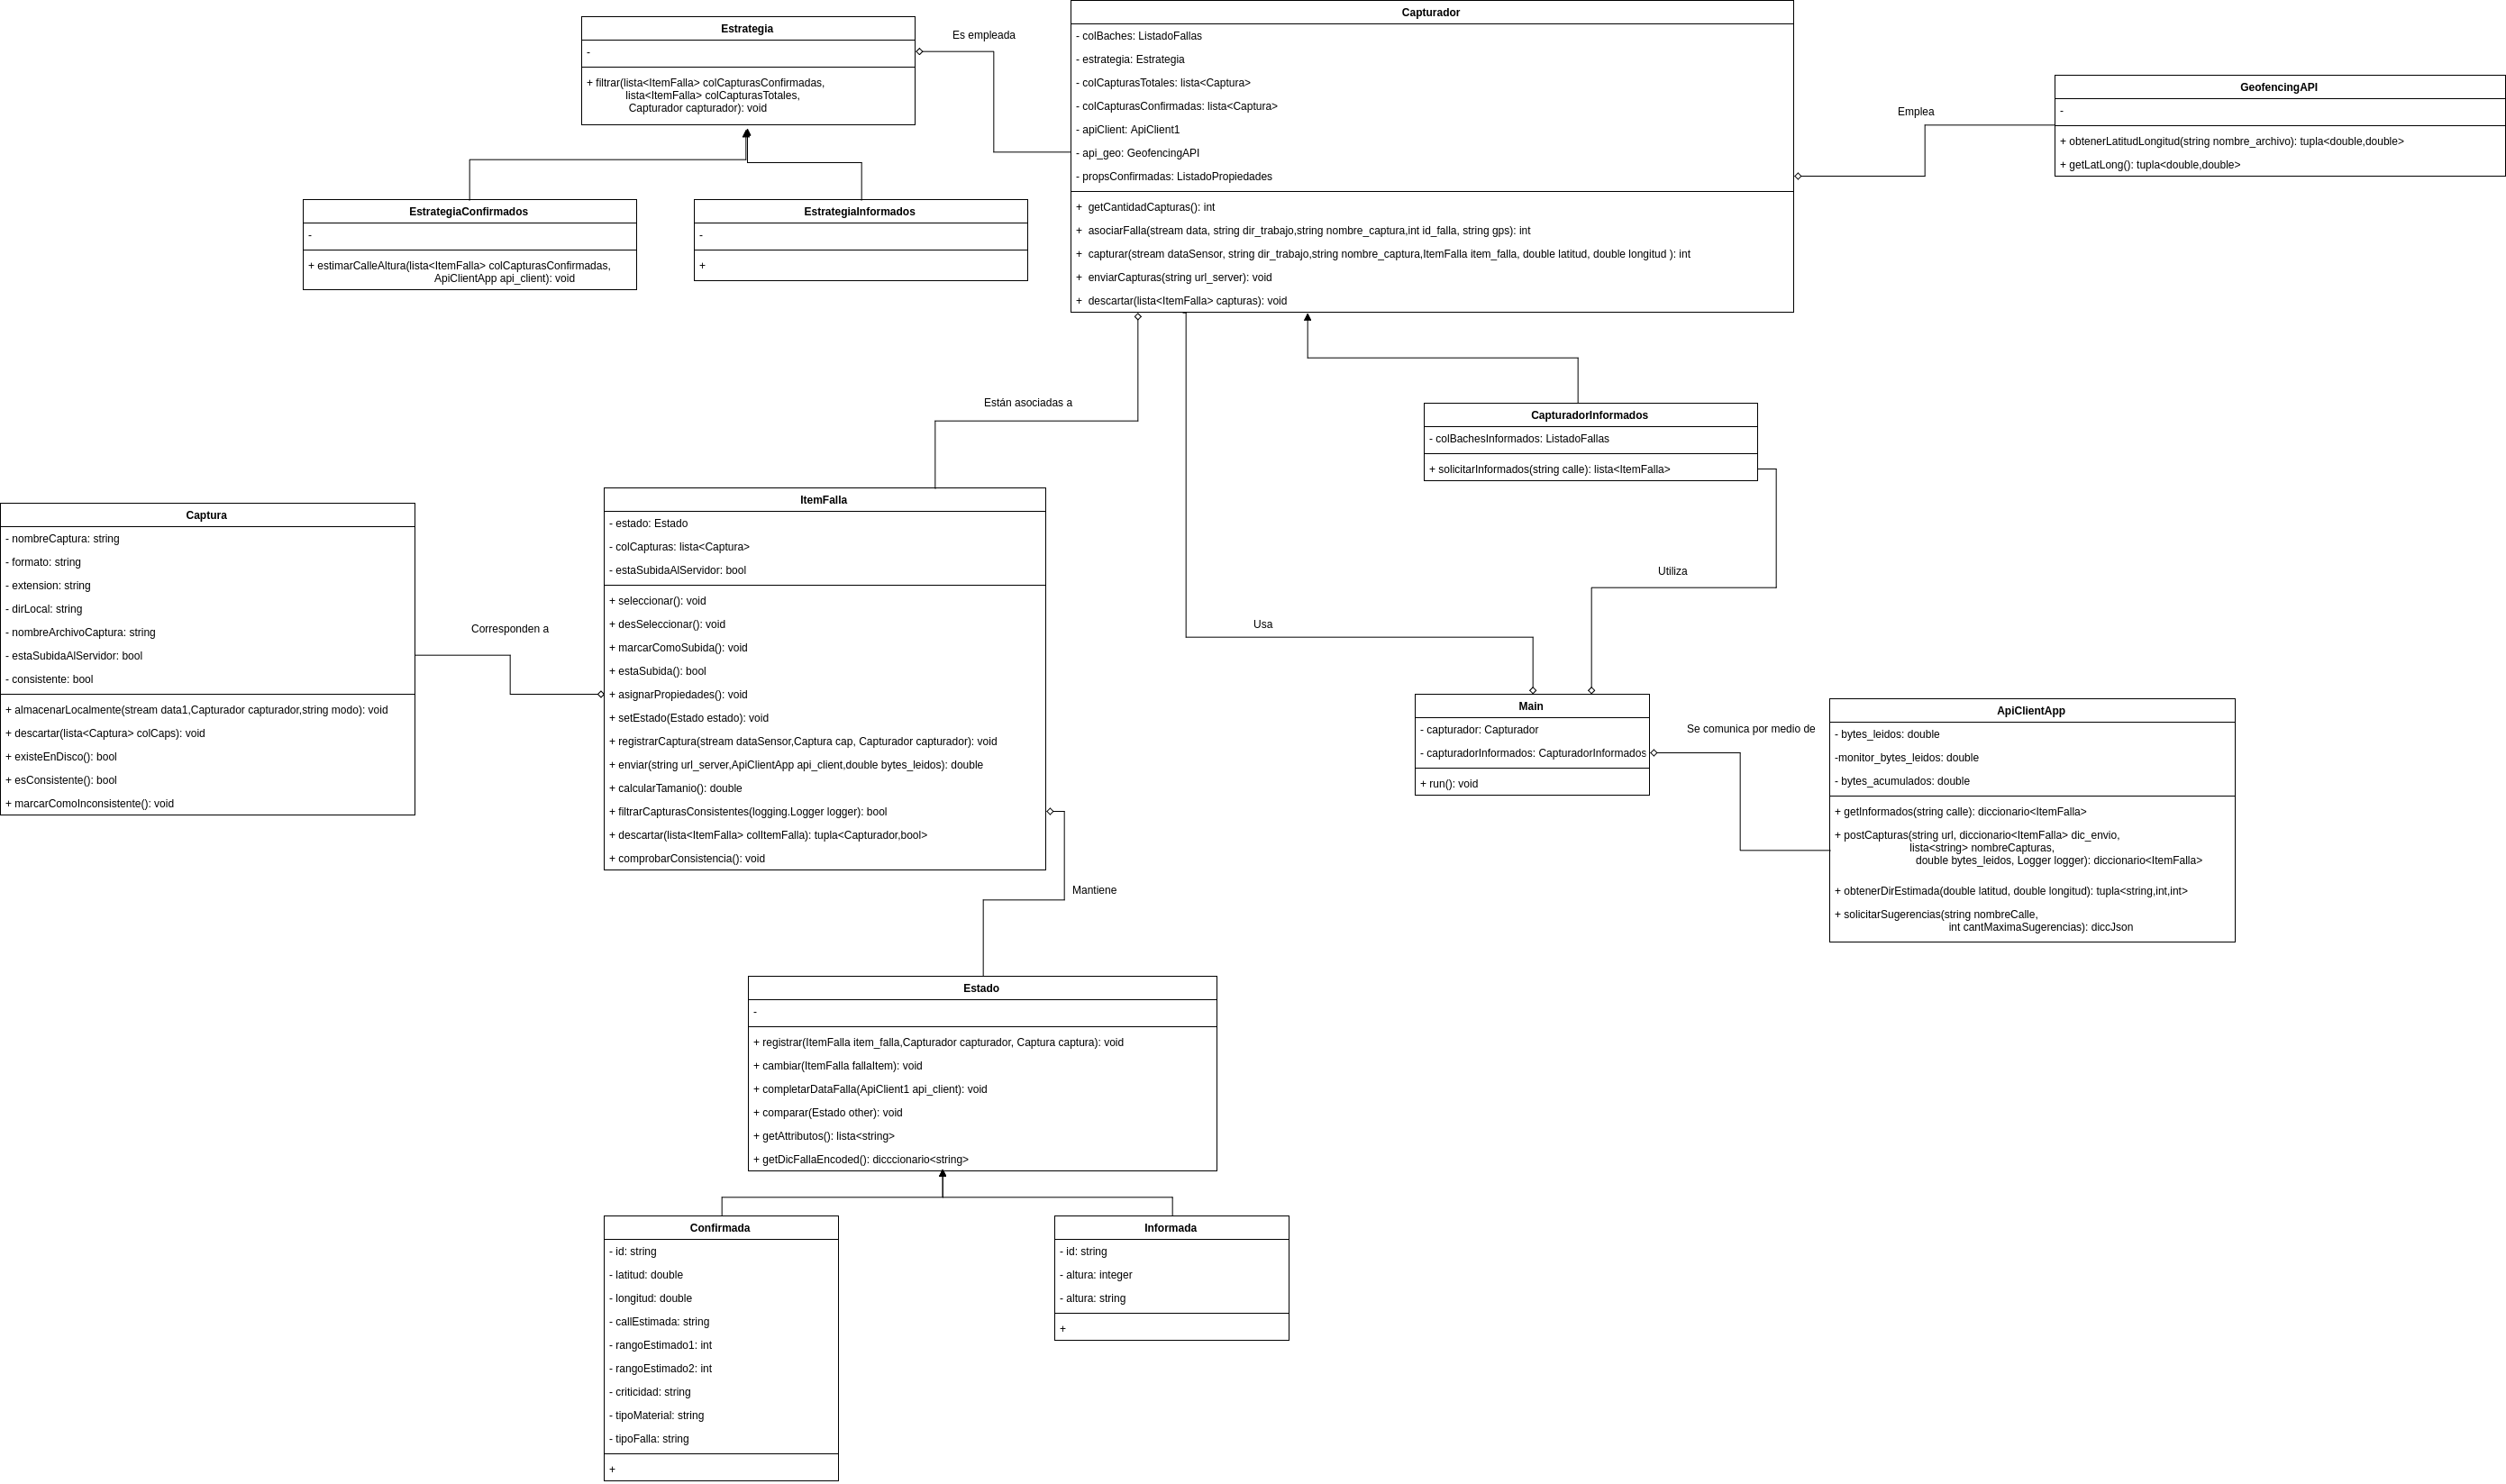
\includegraphics{../figs/Cap6/Final_Diagrama_clases_appCliente.png}
\end{figure}

\newpage
\thispagestyle{my_landscape}
\begin{figure}
  \caption{Diagrama de clases del clasificador}
  \centering
  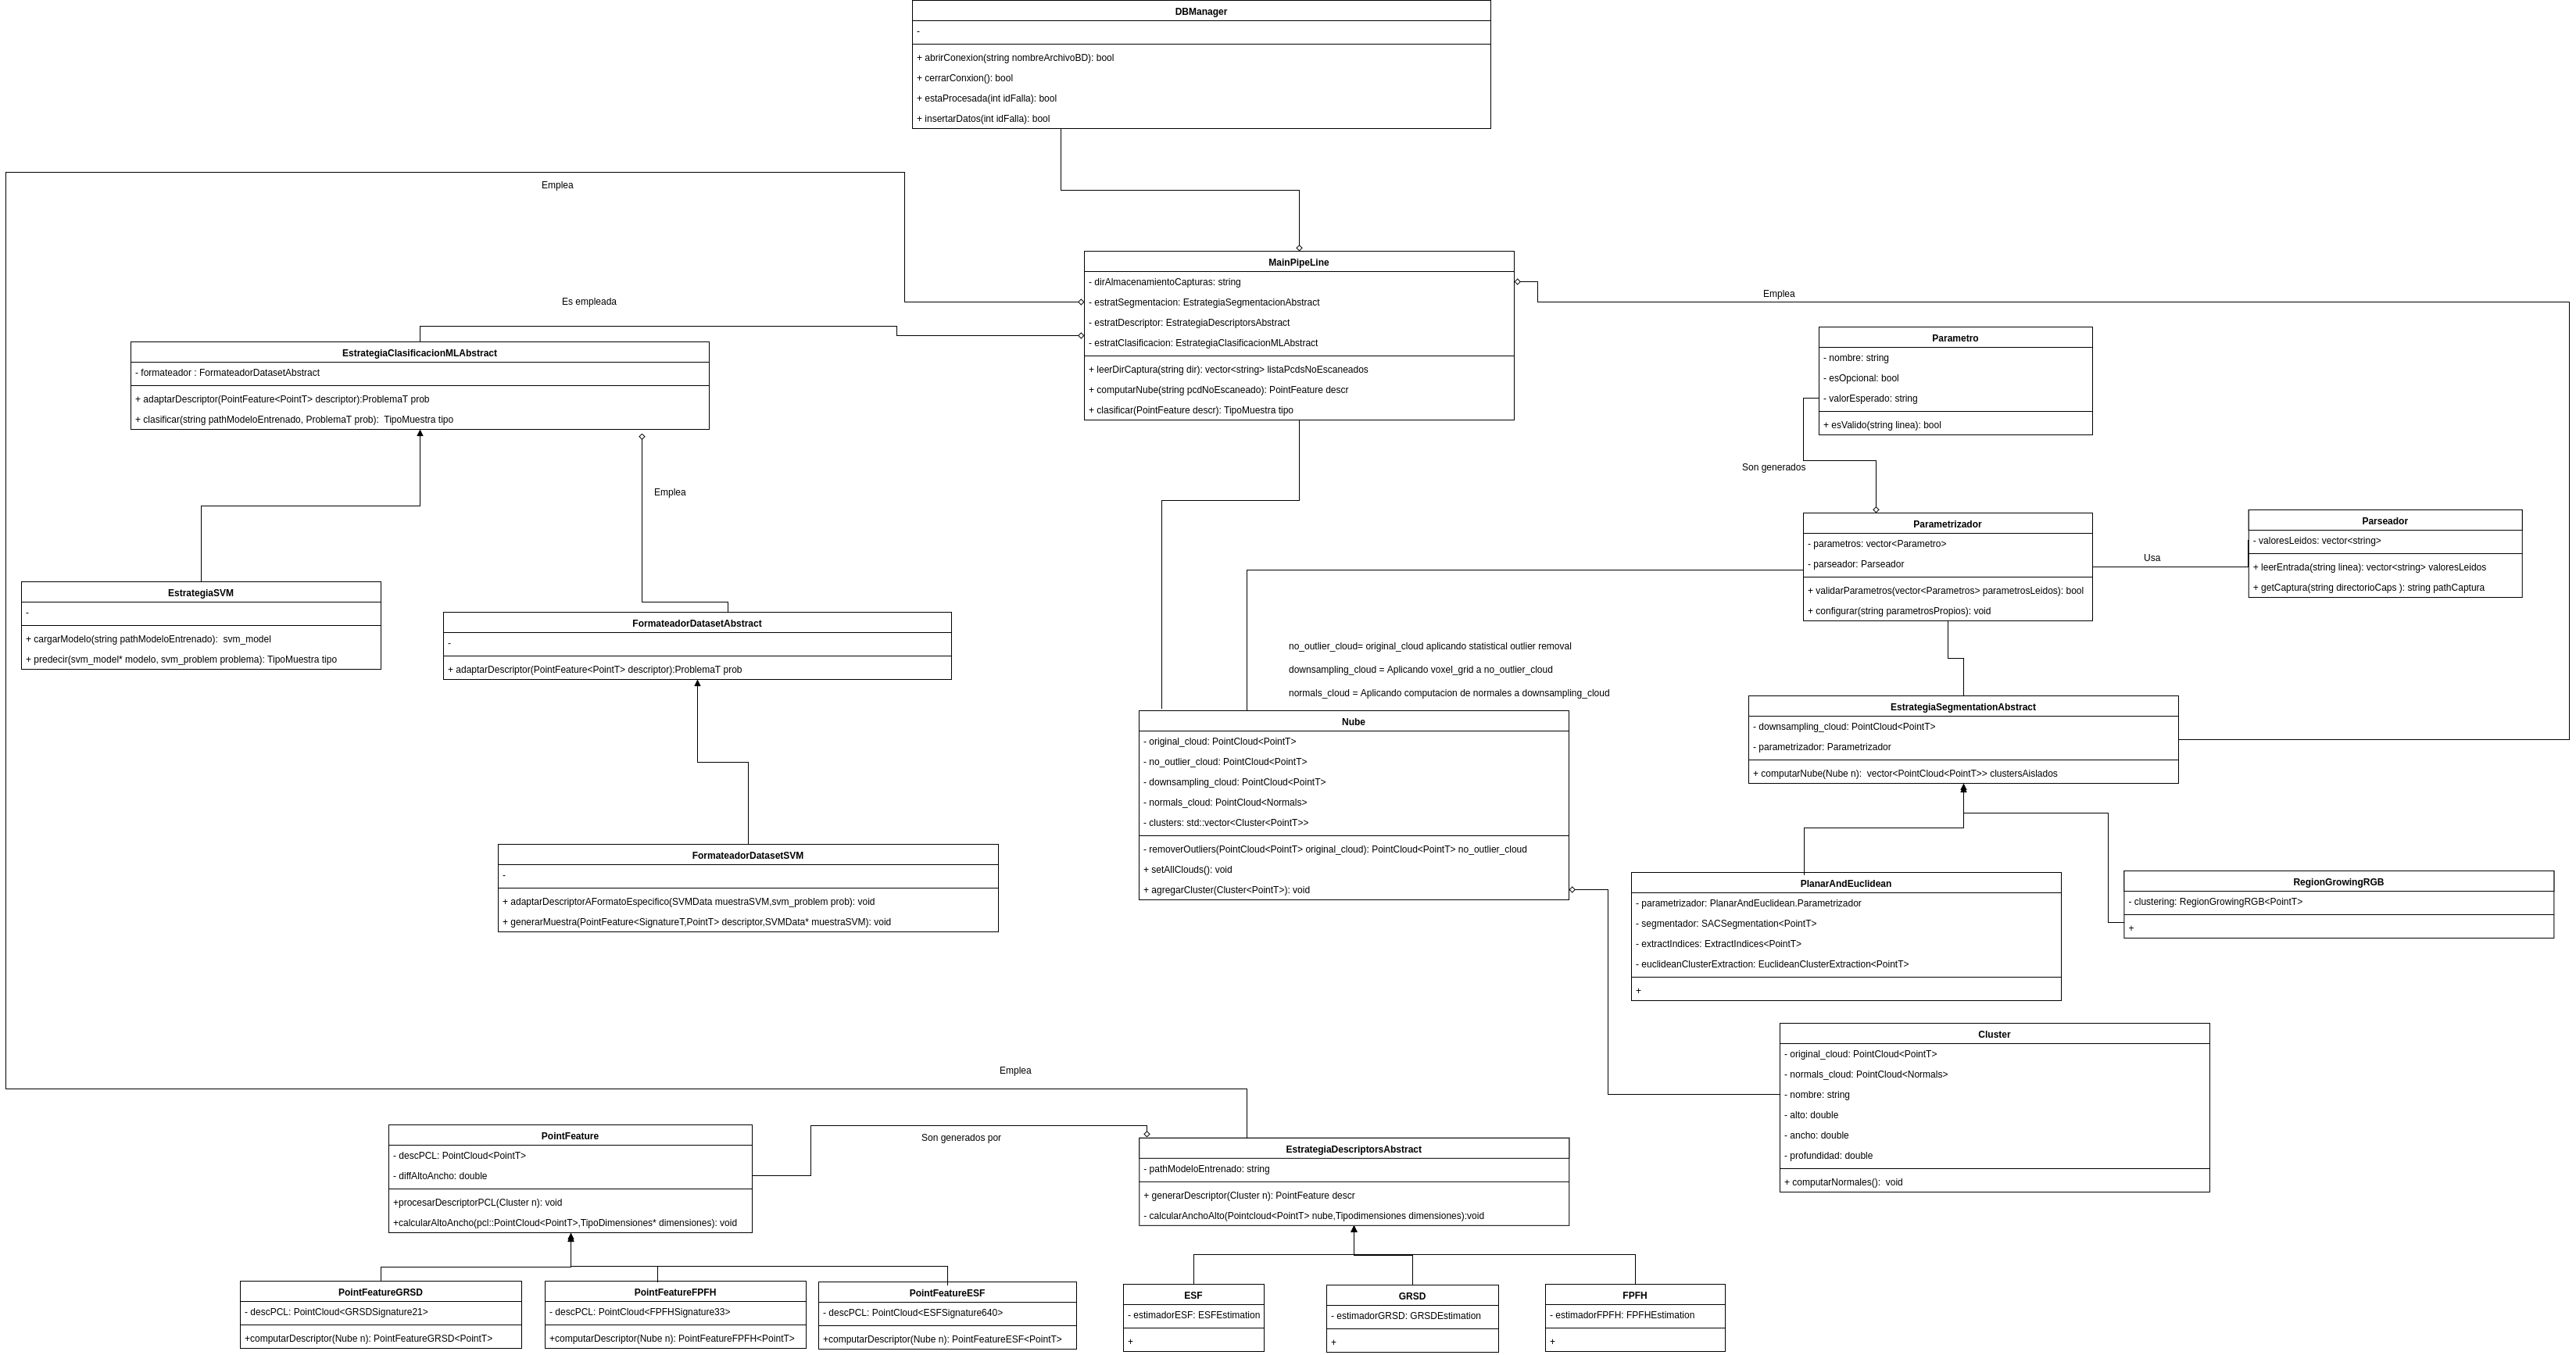
\includegraphics{../figs/Cap6/Final_Diagrama_de_clases_clasificador.png}
\end{figure}

\end{landscape}
\restoregeometry